 \documentclass[11pt,a4paper,onecolumn]{article}
% \documentclass[options]{class}
% Example: \documentclass[11pt,twoside,a4paper]{article} 10 pt is by default.

\setlength{\columnsep}{1cm}
 

\usepackage[T1]{fontenc}       % Use modern font encodings
% \usepackage[version=3]{mhchem} % Formula subscripts using \ce{}
\usepackage{graphicx}
\usepackage[a4paper,top=2cm, bottom=2.5cm, left=2.5cm, right=2.5cm]{geometry}
% \usepackage{authblk} % For affiliation. This package is not preinstalled.
\graphicspath{{./sup_info/}}
\newcommand*\commentauthor[1]{\textbf{{\textit{#1}}}}
\newcommand*\me[1]{\ensuremath{\bar{#1}\,}}
\newcommand*\chem[1]{\ensuremath{\mathrm{#1}}}

\newcommand*{\affaddr}[1]{#1} % No op here. Customize it for different styles.
\newcommand*{\affmark}[1][*]{\textsuperscript{#1}}
\newcommand*{\email}[1]{\texttt{#1}} % These three commands are for author affilations.

\linespread{1.3} % Line spacing. 1.3 means one-and-a-half spacing.

\begin{document}

%\author{
%Biswajit Pradhan, Sebastiaan Van Mulken, Xueyan Miao, Gerard Canters, Michel Orrit\\\affaddr{Huygens-Kamerlingh Onnes Laboratory, Leiden University, 2300 RA Leiden, Netherlands}\\\email{orrit@physics.leidenuniv.nl}
%}

\date{\vspace{1ex}} % Exclude date in the title.
%\affiliation
 %\affil{Huygens-Kamerlingh Onnes Laboratory, Leiden University, 2300 RA Leiden, Netherlands} % This is only useful for authblk package.
 %\email{orrit@leidenuniv.nl}
\title{\textbf{Single azurin redox switching}\\ \vspace{3ex} Supplementary Information \vspace{3ex}}
\maketitle
\tableofcontents
\pagebreak

%\section{Time traces}
%time trace Zn and Cu azurin
\begin{figure}
  \centering
  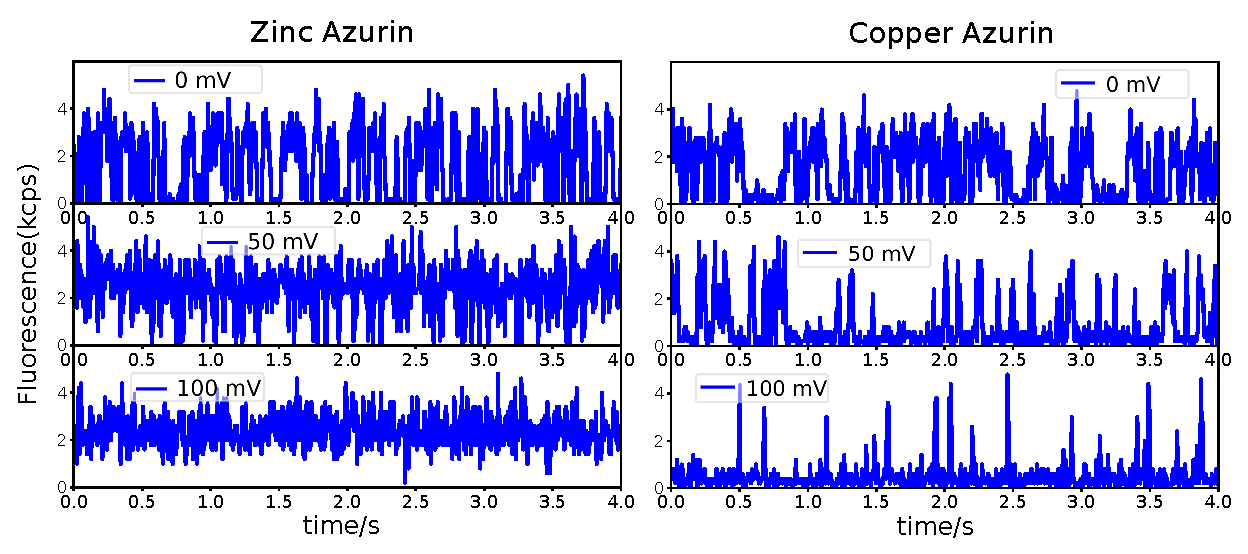
\includegraphics[width=\textwidth,keepaspectratio]{Figure_SI/SI_timetrace_Zn_Cu.eps}
	\makeatletter
	\renewcommand{\fnum@figure}{\figurename~S\thefigure}
	\makeatother
  \caption{Time traces of Zn Azurin (left) and of Cu Azurin(right) labeled with ATTO655 at different potential.  Above 25 mV, Cu-Azurin show swiching in the intensity due to changes in the oxidation state of the Copper metal center and below 25 mV, triplet blinking contributes to the switching as can be seen in the redox inactive Zn-Azurin.}
  \label{SIfig:tracecomparision}
\end{figure}
%mid point potential of ZnAzurin
\begin{figure}
  \centering
  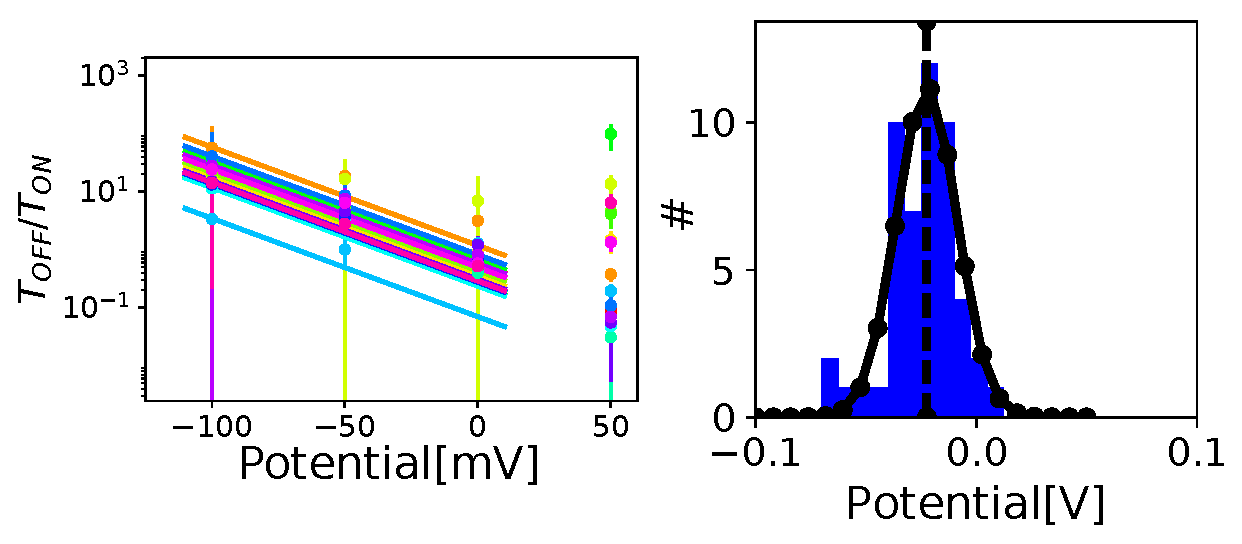
\includegraphics[width=\textwidth,keepaspectratio]{Figure_SI/SI_potential_Zn.eps}
	\makeatletter
	\renewcommand{\fnum@figure}{\figurename~S\thefigure}
	\makeatother
  \caption{\textbf{Zn-AzurinATTO655 blinking.} Ratio between on and off time as a function of applied potential for the same single $ZnAzurin$ molecule. Different color represents different single-molecules. And the line connecting the data points is the Nernst fit for all the data points above 25 mV. The plot in the right is the histogram of midpoint potentials for $51$ molecules with a gaussian fit with center -23 mV with respect to calomel electrode.}
  \label{SIfig:2Dhist_Zn}
\end{figure}
%2D on_off hist: ZnAzurin
\begin{figure}
  \centering
  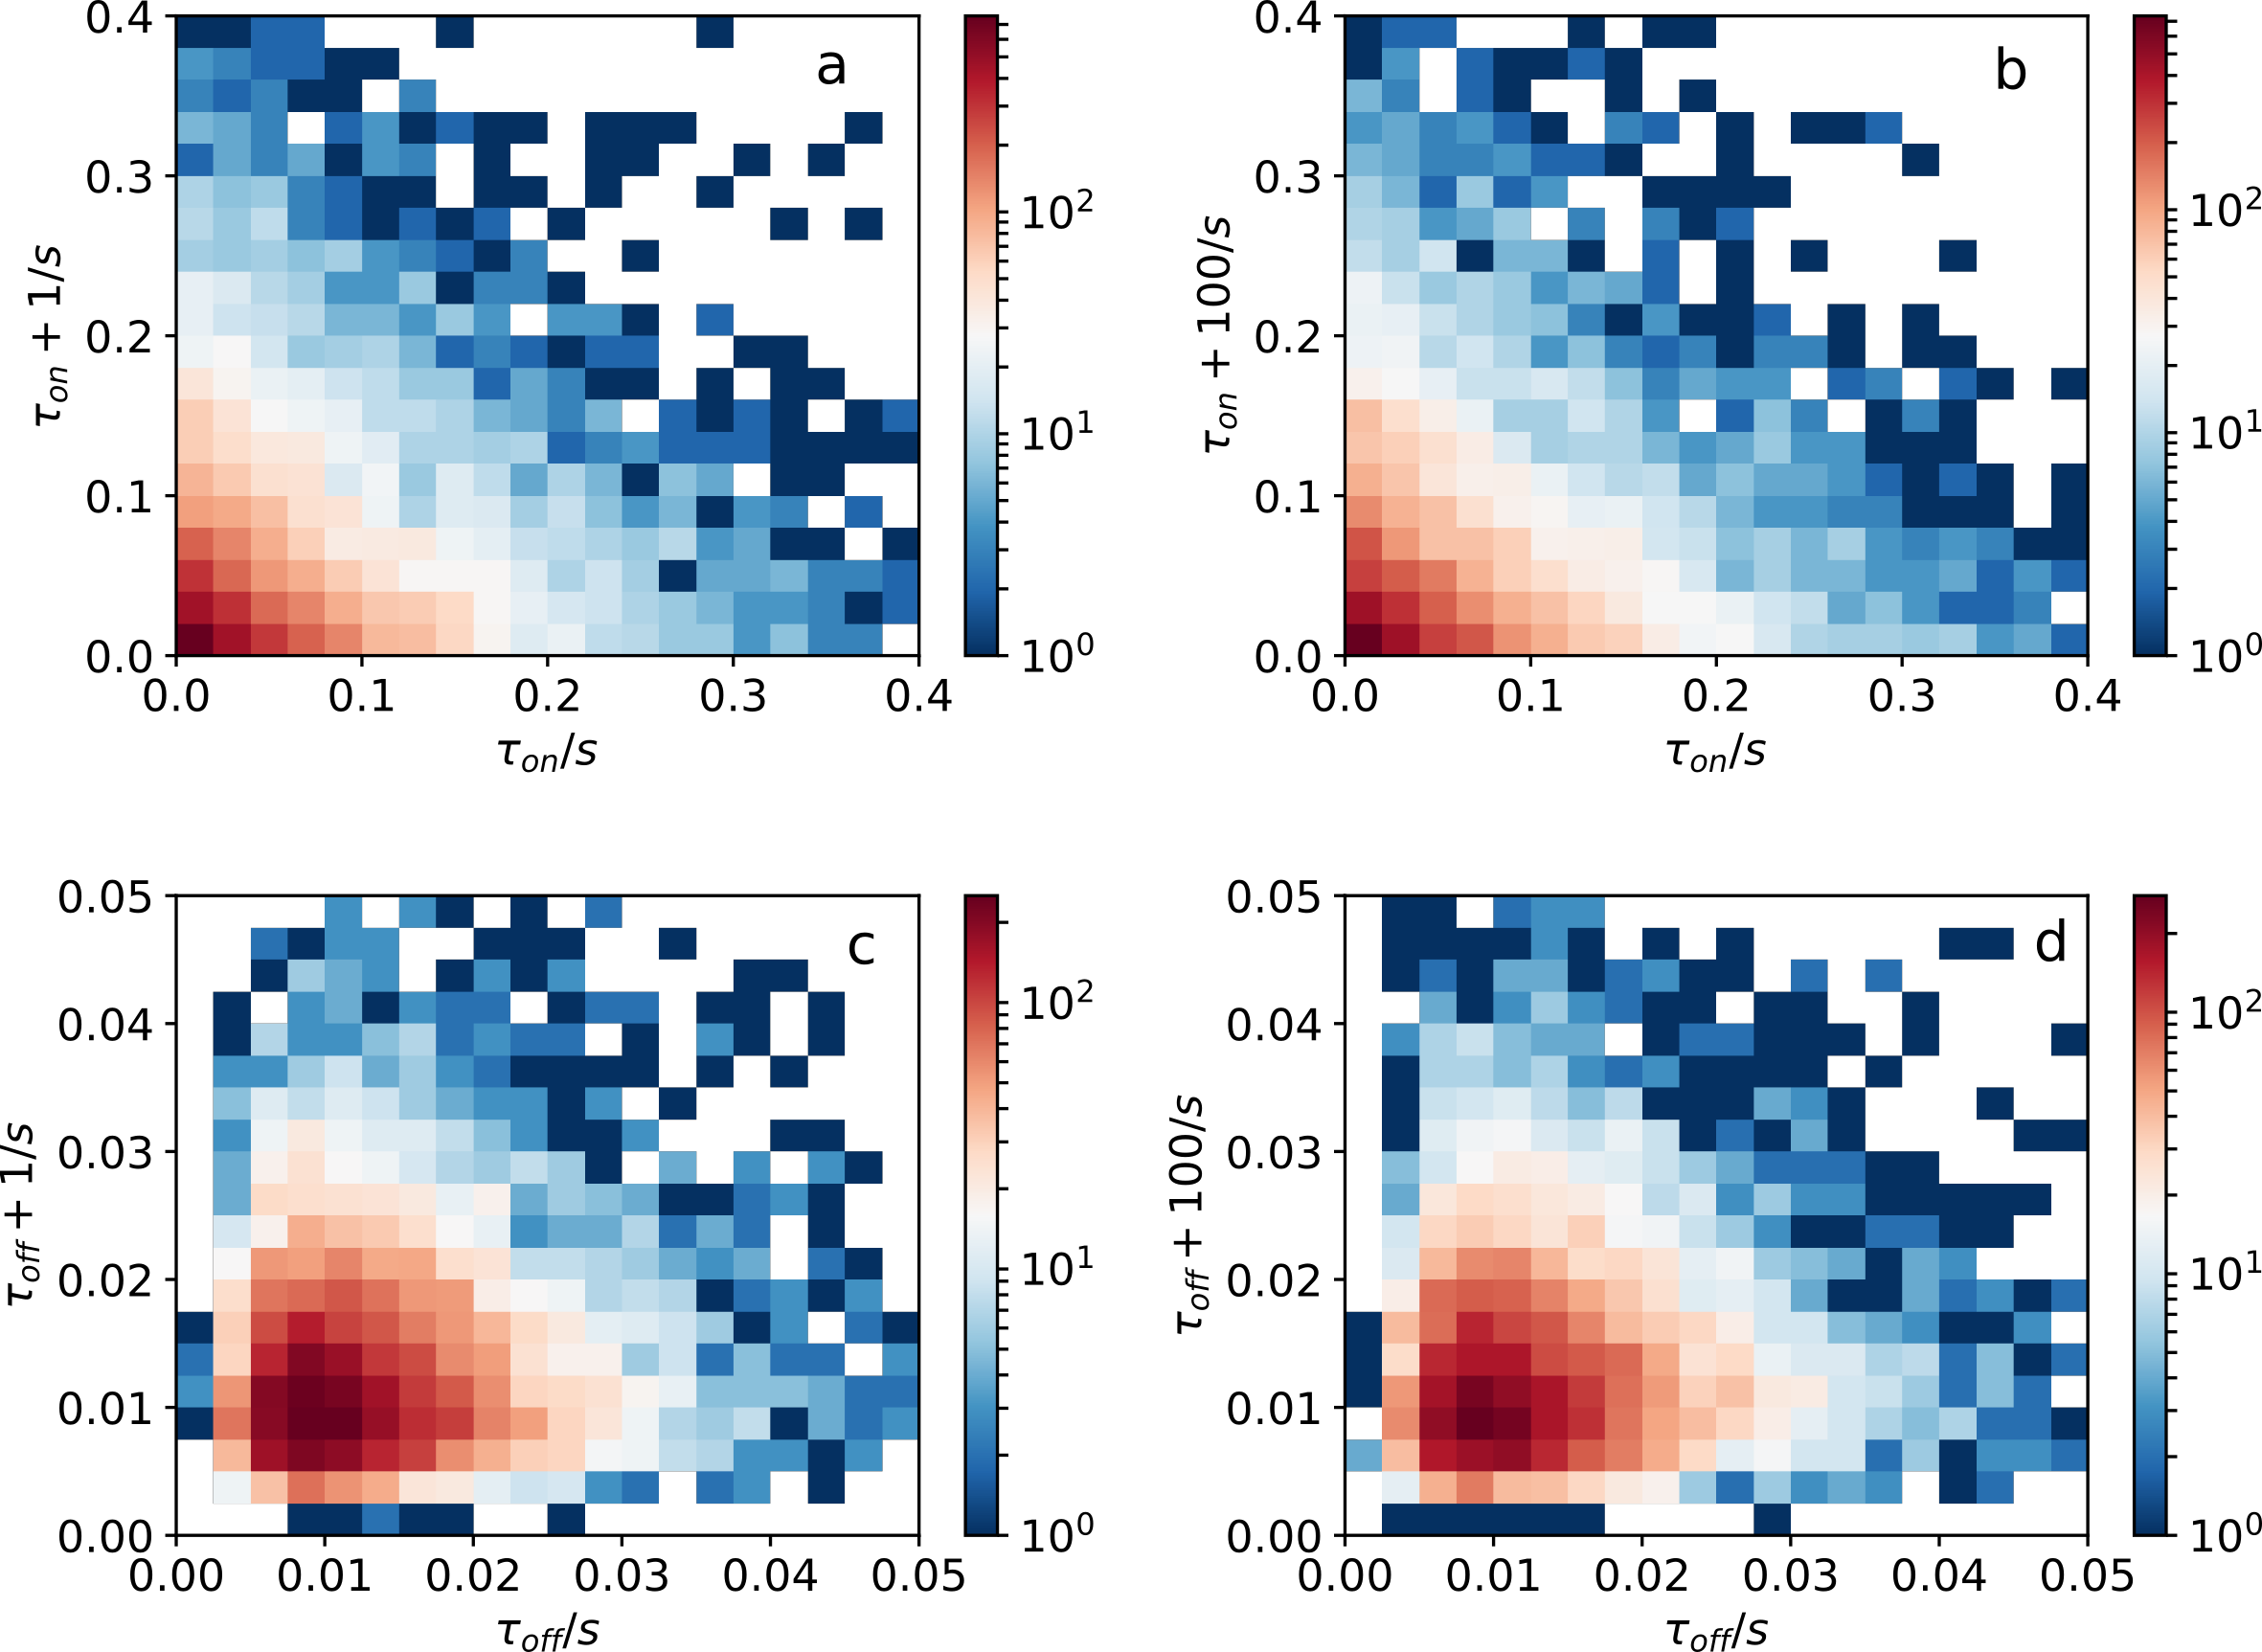
\includegraphics[width=\textwidth,keepaspectratio]{Figure_SI/SI_on_off_2D_histogram_Zn.png}
	\makeatletter
	\renewcommand{\fnum@figure}{\figurename~S\thefigure}
	\makeatother
  \caption{\textbf{2D histogram: Zn-Azurin.} 2D correlation plot of (a) on-times vs the next on-times (b) on-times vs the on-time after 100 turnovers (c) off-times vs next off-times (d) off-times vs the off-time after 100 turnovers.}
  \label{SIfig:tracecomparision}
\end{figure}
%Slope: Nernst equation
\begin{figure}
  \centering
  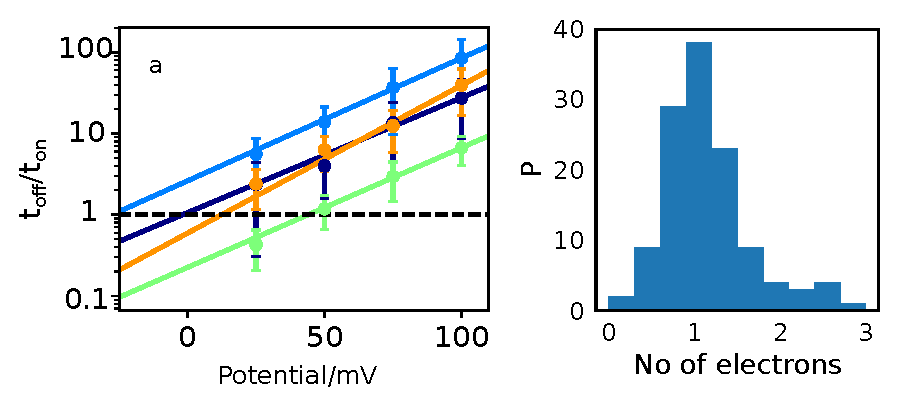
\includegraphics[width=\textwidth,keepaspectratio]{Figure_SI/SI_potential_slope.eps}
	\makeatletter
	\renewcommand{\fnum@figure}{\figurename~S\thefigure}
	\makeatother
  \caption{Fitting with Nernst equation with slope as variable parameters for  (a) Cu-Azurin ATTO655 (b) Zn-Azurin ATTO 655. The corresponding histogram of slopes obtained from the fitting shown in the right.}
  \label{SIfig:potential_slope}
\end{figure}
%\bibliography{}


\end{document}
